\section{Use Cases}
The three proposed visualizations~(cf. Section~\ref{visualizations}) are evaluated by presenting an exemplary use case each visualization helps to solve, based on the questions we identified in Table~\ref{table-questions} in Section~\ref{introduction}.

\subsection{Seasonality in Road Accidents}
\begin{figure}
    \centering
    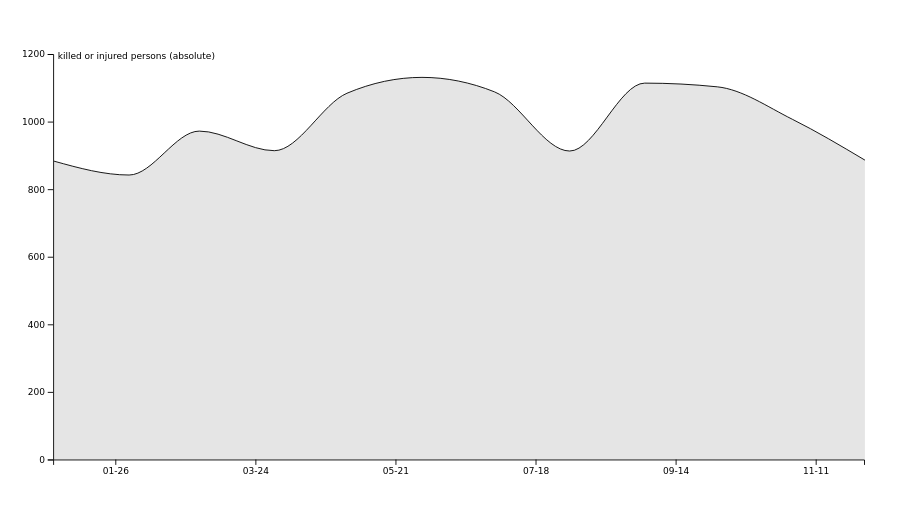
\includegraphics[width=0.9\linewidth]{figures/time-series-2-to-1-killed-or-injured-absolute-by-year-per-month.png}
    \caption{Time series of the number of killed or injured persons per month with a 2:1~aspect ratio, by aggregating across all years~2005--2010.}
    \label{figure-time-series-killed-injured-by-year-per-month}
\end{figure}
An interesting use case for the time series plot is to answer the question whether there is a seasonal influence on the prevalence and severity of road accidents. A citizen living in Paris might ask the following: \enquote{Are roads more dangerous in winter or summer?}
By aggregating injured or killed persons across recent years~(2005--2020) and grouping per month, we get the time series visualization in Figure~\ref{figure-time-series-killed-injured-by-year-per-month}. To be able to spot seasonal trends, we also enable banking to 45\(^\circ\). First, we observe that the monthly number of injured or killed persons is above~800 for all months. But even though one could intuitively think driving in winter would be more dangerous, from December to March there are fewer road casualties.
Because the citizen lives in Paris, they would like to check whether the findings also hold true when only considering accidents from the Paris metropolitan area.
Therefore they switch to the map view to select a grouping by Departements and click on their Departement of Paris. 
With our current implementation this use case faces two difficulties: \Ni because Paris is divided into several Departements, it can be difficult to select the correct Departement from the map and \Nii becuase of the sampling described in Section~\ref{data} the selected sub-set is to small to observe any trends in the time series plot.
In future work, we plan to improve this interaction by optimizing the application code to work with the whole dataset.
Arguably the citizen could also find this seasonal influence in a recursive pattern visualization. But the color mapping of the recursive pattern technique would make it difficult, especially for color-blind people, to distinguish and quantify the extent of seasonality.

\subsection{Second Visualization Use Case}
\todo{Präsentieren sie für jede der drei Visualisierungen einen sinnvollen Anwendungsfall in dem ein bestimmter Fakt, ein Muster oder die Abwesenheit eines Musters visuell festgestellt wird. Begründen Sie, warum dieser Anwendungsfall wichtig für die Zielgruppe der Anwenderinnen ist. Diskutieren Sie weiterhin, ob die oben beschriebene Information auch mit anderen Visualisierungstechniken hätte gefunden werden können. Falls dies möglich wäre, vergleichen sie die den Aufwand und die Schwierigkeiten ihres Ansatzes und möglicher Alternativen.}

\subsection{Third Visualization Use Case}
\todo{Präsentieren sie für jede der drei Visualisierungen einen sinnvollen Anwendungsfall in dem ein bestimmter Fakt, ein Muster oder die Abwesenheit eines Musters visuell festgestellt wird. Begründen Sie, warum dieser Anwendungsfall wichtig für die Zielgruppe der Anwenderinnen ist. Diskutieren Sie weiterhin, ob die oben beschriebene Information auch mit anderen Visualisierungstechniken hätte gefunden werden können. Falls dies möglich wäre, vergleichen sie die den Aufwand und die Schwierigkeiten ihres Ansatzes und möglicher Alternativen.}
